\documentclass[aspectratio=169,10pt]{beamer}

\usetheme{default}
\usefonttheme{professionalfonts}
\setbeamertemplate{navigation symbols}{}
\setbeamertemplate{itemize items}[circle]
\setbeamertemplate{enumerate items}[default]
\setbeamertemplate{blocks}[rounded][shadow=false]

\usepackage[T1]{fontenc}
\usepackage[utf8]{inputenc}
\usepackage{lmodern}
\usepackage{amsmath,amssymb}
\usepackage{booktabs}
\usepackage{array}
\usepackage{tikz}
\usetikzlibrary{arrows.meta,positioning,calc,shapes.geometric,fit}
\usepackage{graphicx}

\definecolor{ink}{HTML}{102A43}
\definecolor{muted}{HTML}{627D98}
\definecolor{paper}{HTML}{F7FAFC}
\definecolor{teal}{HTML}{007C83}
\definecolor{sky}{HTML}{2C7FB8}
\definecolor{lime}{HTML}{52B788}
\definecolor{gold}{HTML}{F4A261}
\definecolor{coral}{HTML}{E76F51}
\definecolor{softteal}{HTML}{D8F3F0}
\definecolor{softgold}{HTML}{FFF1D6}

\setbeamercolor{normal text}{fg=ink,bg=paper}
\setbeamercolor{structure}{fg=teal}
\setbeamercolor{frametitle}{fg=ink,bg=paper}
\setbeamercolor{title}{fg=ink}
\setbeamercolor{subtitle}{fg=muted}
\setbeamercolor{author}{fg=muted}
\setbeamercolor{date}{fg=muted}
\setbeamercolor{alerted text}{fg=coral}
\setbeamercolor{block title}{fg=ink,bg=softteal}
\setbeamercolor{block body}{fg=ink,bg=white}
\setbeamercolor{footline}{fg=muted,bg=paper}
\setbeamerfont{title}{series=\bfseries,size=\Huge}
\setbeamerfont{frametitle}{series=\bfseries,size=\Large}
\setbeamerfont{subtitle}{size=\large}
\setbeamerfont{footnote}{size=\tiny}

\setbeamertemplate{frametitle}{%
  \vspace{0.25cm}\insertframetitle\par
  \vspace{0.08cm}\color{teal}\rule{0.9\linewidth}{0.5pt}\color{ink}
}
\setbeamertemplate{footline}{%
  \hspace{0.55cm}\insertshorttitle\hfill
  \insertsection\hspace{0.3cm}\textcolor{teal}{\insertframenumber/\inserttotalframenumber}\hspace{0.55cm}\vspace{0.16cm}
}

\newcommand{\smallcite}[1]{\par\vspace{0.14cm}{\scriptsize\color{muted}#1}}
\newcommand{\pill}[1]{\tikz[baseline=(X.base)]\node[fill=softteal,rounded corners=3pt,inner xsep=5pt,inner ysep=2pt] (X) {\scriptsize\color{ink}#1};}

\title[HAR progress report]{Progress update: smartphone activity classification}
\subtitle{Milestone 1: reproducible baselines and a one-class GLRT classifier}
\author{SDET Project}
\date{October 2026}

\begin{document}

% 1
\begin{frame}[plain]
  \vspace{0.65cm}
  \begin{tikzpicture}[remember picture,overlay]
    \fill[softteal] (8.9,-0.2) circle (3.25cm);
    \fill[softgold] (10.7,5.9) circle (1.55cm);
    \draw[teal,line width=1.1pt] (9.2,1.25) .. controls (9.65,2.2) and (10.05,0.75) .. (10.55,1.85)
      .. controls (10.95,2.7) and (11.35,1.2) .. (11.8,2.2);
  \end{tikzpicture}
  \titlepage
\end{frame}

% 2
\section{Classification goal}
\begin{frame}{The question behind the project}
  \begin{columns}[T,onlytextwidth]
    \begin{column}{.53\textwidth}
      \vspace{0.2cm}
      \begin{block}{Practical question}
        Can a phone classify an inertial-sensor window as still or moving using only accelerometer measurements?
      \end{block}
      \vspace{0.25cm}
      \uncover<2->{
      \begin{itemize}
        \item The current task is binary classification: \textit{still} versus \textit{moving}.
        \item The eventual task is six-class activity classification.
        \item This project starts with an interpretable one-class GLRT classifier for the binary task.
      \end{itemize}}
    \end{column}
    \begin{column}{.42\textwidth}
      \centering
      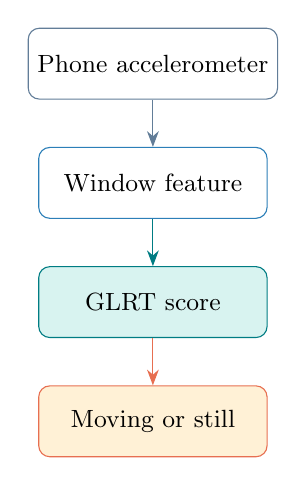
\begin{tikzpicture}[node distance=6mm, every node/.style={font=\small,align=center}]
        \node[draw=muted,rounded corners=4pt,fill=white,minimum width=2.9cm,minimum height=.9cm] (raw) {Phone accelerometer};
        \node[draw=sky,rounded corners=4pt,fill=white,below=of raw,minimum width=2.9cm,minimum height=.9cm] (feature) {Window feature};
        \node<2->[draw=teal,rounded corners=4pt,fill=softteal,below=of feature,minimum width=2.9cm,minimum height=.9cm] (glr) {GLRT score};
        \node<3->[draw=coral,rounded corners=4pt,fill=softgold,below=of glr,minimum width=2.9cm,minimum height=.9cm] (prediction) {Moving or still};
        \draw[-{Stealth[length=2mm]},muted] (raw) -- (feature);
        \draw<2->[-{Stealth[length=2mm]},teal] (feature) -- (glr);
        \draw<3->[-{Stealth[length=2mm]},coral] (glr) -- (prediction);
      \end{tikzpicture}
    \end{column}
  \end{columns}
\end{frame}

% 3
\begin{frame}{What the literature tells us}
  \begin{columns}[T,onlytextwidth]
    \begin{column}{.48\textwidth}
      \begin{block}{Human activity recognition foundations}
        \begin{itemize}
          \item Smartphone inertial signals can distinguish common daily activities.\cite{anguita2013}
          \item WISDM established an early phone-accelerometer benchmark for six activities.\cite{kwapisz2011}
          \item Window length shapes both recognition accuracy and response latency.\cite{banos2014}
        \end{itemize}
      \end{block}
    \end{column}
    \begin{column}{.48\textwidth}
      \begin{block}{Why a GLRT classifier}
        \begin{itemize}
          \item A generalized likelihood-ratio test compares how well competing statistical hypotheses explain a window.\cite{basseville1993}
          \item It gives an interpretable binary decision without training a complex deep network.
          \item Our contribution so far is a reproducible one-class GLRT classifier, not a six-class classifier.
        \end{itemize}
      \end{block}
    \end{column}
  \end{columns}
\end{frame}

% 4
\section{Data}
\begin{frame}{Two complementary public datasets}
  \begin{columns}[T,onlytextwidth]
    \begin{column}{.48\textwidth}
      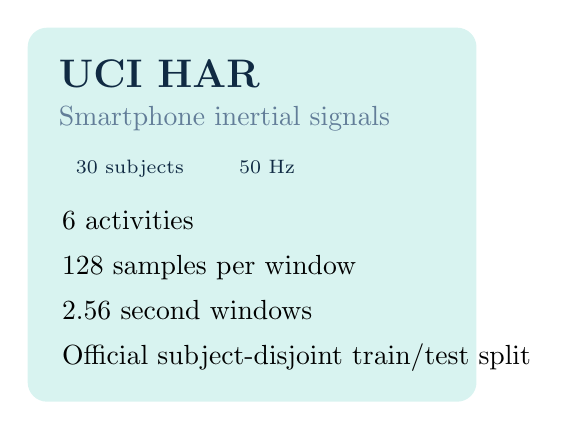
\begin{tikzpicture}
        \node[fill=softteal,rounded corners=7pt,minimum width=5.7cm,minimum height=4.75cm,anchor=north west] at (0,0) {};
        \node[anchor=north west,font=\Large\bfseries,text=ink] at (.28,-.3) {UCI HAR};
        \node[anchor=north west,text=muted] at (.28,-.88) {Smartphone inertial signals};
        \node[anchor=north west,align=left] at (.32,-1.5) {\pill{30 subjects}\quad \pill{50 Hz}\\[.28cm]
          6 activities\\[.15cm]
          128 samples per window\\[.15cm]
          2.56 second windows\\[.15cm]
          Official subject-disjoint train/test split};
      \end{tikzpicture}
    \end{column}
    \begin{column}{.48\textwidth}
      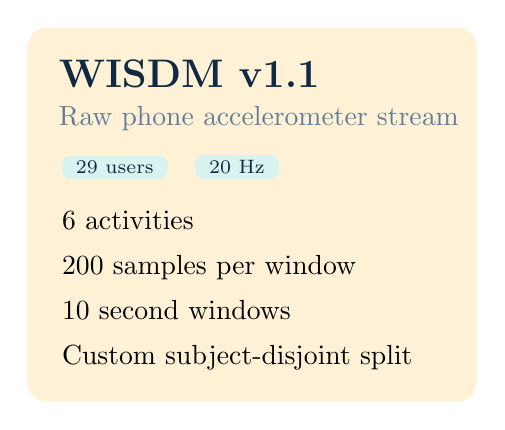
\begin{tikzpicture}
        \node[fill=softgold,rounded corners=7pt,minimum width=5.7cm,minimum height=4.75cm,anchor=north west] at (0,0) {};
        \node[anchor=north west,font=\Large\bfseries,text=ink] at (.28,-.3) {WISDM v1.1};
        \node[anchor=north west,text=muted] at (.28,-.88) {Raw phone accelerometer stream};
        \node[anchor=north west,align=left] at (.32,-1.5) {\pill{29 users}\quad \pill{20 Hz}\\[.28cm]
          6 activities\\[.15cm]
          200 samples per window\\[.15cm]
          10 second windows\\[.15cm]
          Custom subject-disjoint split};
      \end{tikzpicture}
    \end{column}
  \end{columns}
  \vfill
  \smallcite{UCI HAR: Anguita et al.\ \cite{anguita2013}. WISDM: Kwapisz et al.\ \cite{kwapisz2011}.}
\end{frame}

% 5
\begin{frame}{The first classification task is deliberately coarse}
  \centering
  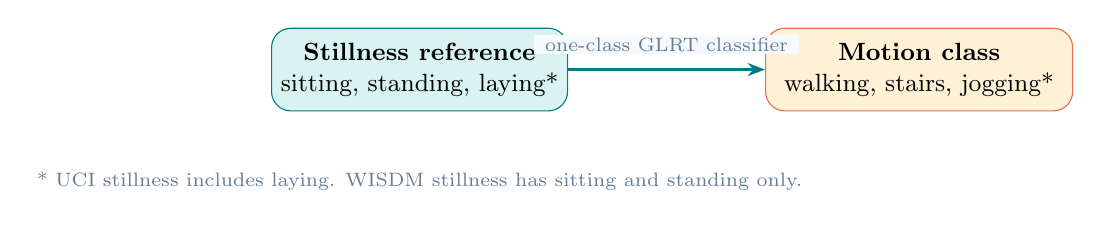
\begin{tikzpicture}[every node/.style={font=\small,align=center}]
    \node[draw=teal,fill=softteal,rounded corners=7pt,minimum width=3.0cm,minimum height=1.05cm] (still) {\textbf{Stillness reference}\\sitting, standing, laying*};
    \node[draw=coral,fill=softgold,rounded corners=7pt,minimum width=3.9cm,minimum height=1.05cm,right=2.5cm of still] (motion) {\textbf{Motion class}\\walking, stairs, jogging*};
    \draw[-{Stealth[length=2.2mm]},line width=1pt,teal] (still) -- node[above=5pt,fill=paper,inner xsep=4pt,inner ysep=1pt,text=muted,font=\scriptsize] {one-class GLRT classifier} (motion);
    \node[below=.65cm of still,text=muted,font=\scriptsize,align=left] {* UCI stillness includes laying. WISDM stillness has sitting and standing only.};
  \end{tikzpicture}
  \vspace{.6cm}
  \begin{columns}[T,onlytextwidth]
    \begin{column}{.48\textwidth}
      \uncover<2->{\begin{block}{What this can establish}
        Whether a window is correctly classified as still or moving.
      \end{block}}
    \end{column}
    \begin{column}{.48\textwidth}
      \uncover<3->{\begin{block}{What it does not establish}
        Six-class recognition or a detailed activity label after a moving prediction.
      \end{block}}
    \end{column}
  \end{columns}
\end{frame}

% 6
\section{Preprocessing}
\begin{frame}{UCI HAR preprocessing}
  \centering
  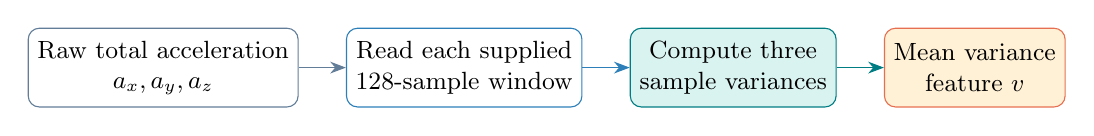
\begin{tikzpicture}[node distance=6mm,every node/.style={font=\small,align=center}]
    \node[draw=muted,fill=white,rounded corners=4pt,minimum width=2.25cm,minimum height=1cm] (a) {Raw total acceleration\\$a_x,a_y,a_z$};
    \node<2->[draw=sky,fill=white,rounded corners=4pt,minimum width=2.25cm,minimum height=1cm,right=of a] (b) {Read each supplied\\128-sample window};
    \node<3->[draw=teal,fill=softteal,rounded corners=4pt,minimum width=2.25cm,minimum height=1cm,right=of b] (c) {Compute three\\sample variances};
    \node<4->[draw=coral,fill=softgold,rounded corners=4pt,minimum width=2.25cm,minimum height=1cm,right=of c] (d) {Mean variance\\feature $v$};
    \draw<2->[-{Stealth[length=2mm]},muted] (a) -- (b);
    \draw<3->[-{Stealth[length=2mm]},sky] (b) -- (c);
    \draw<4->[-{Stealth[length=2mm]},teal] (c) -- (d);
  \end{tikzpicture}
  \vspace{.65cm}
  \begin{block}{Data integrity and split}
    Non-finite feature values are removed only if present, while labels remain aligned. The official UCI train/test partition is retained, so test subjects are not used during calibration.
  \end{block}
  \[
    v = \frac{\operatorname{Var}(a_x)+\operatorname{Var}(a_y)+\operatorname{Var}(a_z)}{3}
  \]
\end{frame}

% 7
\begin{frame}{WISDM preprocessing}
  \begin{columns}[T,onlytextwidth]
    \begin{column}{.60\textwidth}
      \begin{enumerate}
        \item<1-> Recover semicolon-delimited records, including lines containing two records.
        \item<2-> Drop malformed, non-numeric, invalid-activity, and non-finite records.
        \item<3-> Split the stream whenever user or activity changes.
        \item<4-> Form non-overlapping, activity-pure 200-sample windows.
        \item<5-> Discard incomplete remainder samples within each run.
        \item<6-> Hold out users divisible by three for testing; fit on all other users.
      \end{enumerate}
    \end{column}
    \begin{column}{.35\textwidth}
      \centering
      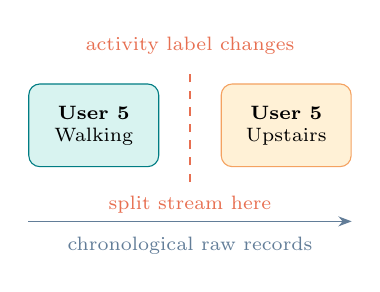
\begin{tikzpicture}[every node/.style={font=\scriptsize,align=center}]
        \node[draw=teal,fill=softteal,rounded corners=4pt,minimum width=1.65cm,minimum height=1.05cm] (run-a) {\textbf{User 5}\\Walking};
        \node[draw=gold,fill=softgold,rounded corners=4pt,minimum width=1.65cm,minimum height=1.05cm,right=.78cm of run-a] (run-b) {\textbf{User 5}\\Upstairs};
        \coordinate (split) at ($(run-a.east)!0.5!(run-b.west)$);
        \draw[coral,dashed,line width=.85pt] ($(split)+(0,-.72cm)$) -- ($(split)+(0,.72cm)$);
        \node[text=coral,above=.78cm of split] {activity label changes};
        \node[text=coral,below=.78cm of split] {split stream here};
        \draw[-{Stealth[length=1.7mm]},muted] ($(run-a.west)+(0,-1.22cm)$) -- ($(run-b.east)+(0,-1.22cm)$);
        \node[text=muted,below=1.3cm of split] {chronological raw records};
      \end{tikzpicture}
      \vspace{.5cm}
      \uncover<6->{\begin{block}{Resulting data}
        5,225 complete windows\\3,597 train, 1,628 test
      \end{block}}
    \end{column}
  \end{columns}
\end{frame}

% 8
\section{Variance threshold baseline}
\begin{frame}{Baseline 1: a transparent variance threshold}
  \begin{columns}[T,onlytextwidth]
    \begin{column}{.55\textwidth}
      \begin{enumerate}
        \item Calculate $v$ for every window.
        \item Fit a threshold on UCI training data only.
        \item Predict moving if $v \geq \tau$, otherwise still.
        \item Select $\tau$ by maximum training balanced accuracy.
      \end{enumerate}
      \vspace{.25cm}
      \uncover<2->{\begin{block}{Why begin here?}
        It is simple enough to audit and establishes whether raw motion energy alone separates the coarse classes.
      \end{block}}
    \end{column}
    \begin{column}{.40\textwidth}
      \centering
      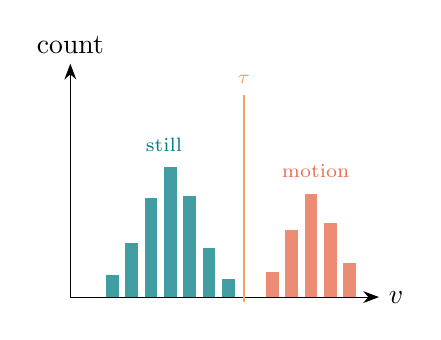
\begin{tikzpicture}[x=.7cm,y=.57cm]
        \draw[-{Stealth[length=2mm]}] (0,0) -- (0,5.2) node[above] {count};
        \draw[-{Stealth[length=2mm]}] (0,0) -- (5.6,0) node[right] {$v$};
        \foreach \x/\h in {.65/.5,1.0/1.2,1.35/2.2,1.7/2.9,2.05/2.25,2.4/1.1,2.75/.4} {\fill[teal!75] (\x,0) rectangle +(.23,\h);}
        \foreach \x/\h in {3.55/.55,3.9/1.5,4.25/2.3,4.6/1.65,4.95/.75} {\fill[coral!80] (\x,0) rectangle +(.23,\h);}
        \draw<2->[gold,line width=1pt] (3.15,-.12) -- (3.15,4.5);
        \node<2->[font=\scriptsize,text=gold,anchor=south] at (3.15,4.55) {$\tau$};
        \node[font=\scriptsize,text=teal] at (1.7,3.4) {still};
        \node[font=\scriptsize,text=coral] at (4.45,2.8) {motion};
      \end{tikzpicture}
    \end{column}
  \end{columns}
\end{frame}

% 9
\begin{frame}{Progress checkpoint: why we moved beyond a fixed threshold}
  \begin{columns}[T,onlytextwidth]
    \begin{column}{.46\textwidth}
      {\scriptsize\color{teal}\textsc{Baseline finding}}\\[.15cm]
      {\large\bfseries A scalar variance threshold is excellent for coarse motion versus stillness.}\\[.45cm]
      {\color{teal}\fontsize{32}{34}\selectfont\textbf{99.90\%}}\\[-.04cm]
      {\scriptsize\color{muted}UCI HAR held-out binary accuracy}\\[.28cm]
      \begin{tabular}{@{}lr@{}}
        \textcolor{muted}{Stillness false-positive rate} & \textbf{0.13\%} \\
        \textcolor{muted}{Confusion errors} & \textbf{3 of 2,947} \\
      \end{tabular}
    \end{column}
    \begin{column}{.06\textwidth}
      \centering\color{softteal}\rule{1pt}{4.0cm}
    \end{column}
    \begin{column}{.46\textwidth}
      {\scriptsize\color{coral}\textsc{Limitation}}\\[.15cm]
      {\large\bfseries The same scalar is not a credible six-class activity recognizer.}\\[.42cm]
      \begin{tabular}{@{}lr@{}}
        \textcolor{muted}{UCI HAR six-class accuracy} & {\color{coral}\large\textbf{37.87\%}} \\
        \textcolor{muted}{WISDM six-class accuracy} & {\color{coral}\large\textbf{58.11\%}} \\
      \end{tabular}\\[.30cm]
      \small\color{muted}Still postures overlap at low variance. Walking and stairs overlap at higher variance.
    \end{column}
  \end{columns}
\end{frame}

% 10
\section{One-class GLRT}
\begin{frame}{What is a generalized likelihood-ratio test?}
  \begin{columns}[T,onlytextwidth]
    \begin{column}{.48\textwidth}
      \begin{block}{Null hypothesis $H_0$}
        The observed window is consistent with the stillness distribution.
      \end{block}
      \vspace{.12cm}
      \uncover<2->{\begin{block}{Alternative hypothesis $H_1$}
        The window is better explained by a higher, unknown motion-related mean.
      \end{block}}
      \vspace{.12cm}
      \uncover<3->{\begin{block}{Decision}
        Classify the window as moving when evidence for $H_1$ exceeds $H_0$ beyond a calibrated threshold.
      \end{block}}
    \end{column}
    \begin{column}{.47\textwidth}
      \centering
      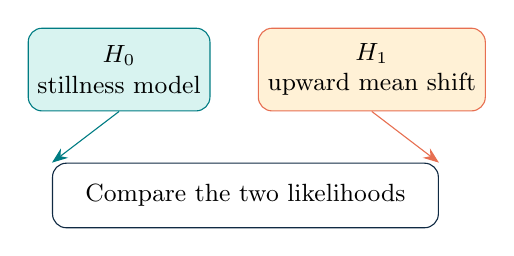
\begin{tikzpicture}[every node/.style={align=center,font=\small}]
        \node[draw=teal,fill=softteal,rounded corners=5pt,minimum width=2.15cm,minimum height=1.05cm] (h0) {$H_0$\\stillness model};
        \node<2->[draw=coral,fill=softgold,rounded corners=5pt,minimum width=2.15cm,minimum height=1.05cm,right=.6cm of h0] (h1) {$H_1$\\upward mean shift};
        \only<3->{%
          \coordinate (mid) at ($(h0.south)!0.5!(h1.south)$);
          \node[draw=ink,fill=white,rounded corners=5pt,minimum width=4.9cm,minimum height=.82cm,below=.65cm of mid] (d) {Compare the two likelihoods};
          \draw[-{Stealth[length=2mm]},teal] (h0.south) -- (d.north west);
          \draw[-{Stealth[length=2mm]},coral] (h1.south) -- (d.north east);
        }
      \end{tikzpicture}
    \end{column}
  \end{columns}
\end{frame}

% 11
\begin{frame}{Our one-class GLRT, step by step}
  \begin{enumerate}
    \item<1-> Keep only \alert{training stillness} windows.
    \item<2-> Transform the positive variance feature: $z=\log(v)$.
    \item<3-> Estimate the stillness reference $z\sim\mathcal{N}(\mu_0,\sigma_0^2)$.
    \item<4-> For each candidate window, calculate the one-sided twice-log likelihood ratio:
  \end{enumerate}
  \vspace{-.05cm}
  \begin{equation*}
    \uncover<4->{G=\max\left(0,\frac{z-\mu_0}{\sigma_0}\right)^2}
  \end{equation*}
  \begin{enumerate}
    \setcounter{enumi}{4}
    \item<5-> Set the decision boundary $h$ from the upper 1\% tail of \alert{training-still} scores.
    \item<6-> Classify the window as moving only when $G>h$.
  \end{enumerate}
  \uncover<7->{\begin{alertblock}{Why one-sided?}
    The project asks whether a stillness reference has shifted upward into motion. Low variance remains compatible with stillness.
  \end{alertblock}}
\end{frame}

% 12
\begin{frame}{From sensor window to GLRT classification}
  \centering
  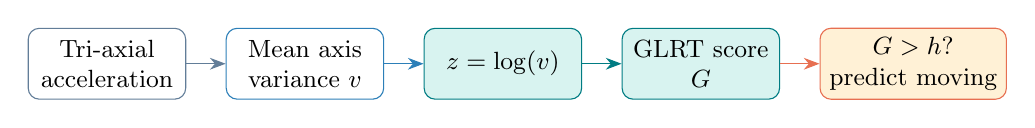
\begin{tikzpicture}[node distance=5mm,every node/.style={font=\small,align=center}]
    \node[draw=muted,fill=white,rounded corners=4pt,minimum width=2.0cm,minimum height=.9cm] (raw) {Tri-axial\\acceleration};
    \node<2->[draw=sky,fill=white,rounded corners=4pt,minimum width=2.0cm,minimum height=.9cm,right=of raw] (var) {Mean axis\\variance $v$};
    \node<3->[draw=teal,fill=softteal,rounded corners=4pt,minimum width=2.0cm,minimum height=.9cm,right=of var] (log) {$z=\log(v)$};
    \node<4->[draw=teal,fill=softteal,rounded corners=4pt,minimum width=2.0cm,minimum height=.9cm,right=of log] (score) {GLRT score\\$G$};
    \node<5->[draw=coral,fill=softgold,rounded corners=4pt,minimum width=2.0cm,minimum height=.9cm,right=of score] (prediction) {$G>h$?\\predict moving};
    \draw<2->[-{Stealth[length=2mm]},muted] (raw) -- (var);
    \draw<3->[-{Stealth[length=2mm]},sky] (var) -- (log);
    \draw<4->[-{Stealth[length=2mm]},teal] (log) -- (score);
    \draw<5->[-{Stealth[length=2mm]},coral] (score) -- (prediction);
  \end{tikzpicture}
  \vspace{.65cm}
  \uncover<6->{\begin{block}{No leakage}
    The mean, standard deviation, and threshold are fitted before evaluation and use no motion labels or held-out-subject data.
  \end{block}}
\end{frame}

% 13
\section{Results}
\begin{frame}{Milestone 1 result: the implemented one-class GLRT classifier}
  \centering\pill{Current implementation: per-window still versus moving classifier}\\[.35cm]
  \renewcommand{\arraystretch}{1.42}
  \begin{tabular}{lrrrr}
    \toprule
    Dataset & Accuracy & Motion recall & Still specificity & Still FPR \\
    \midrule
    UCI HAR & \textbf{99.86\%} & 100.00\% & 99.74\% & 0.26\% \\
    WISDM & \textbf{100.00\%} & 100.00\% & 100.00\% & 0.00\% \\
    \bottomrule
  \end{tabular}
  \vspace{.65cm}
  \begin{columns}[T,onlytextwidth]
    \begin{column}{.47\textwidth}
      \uncover<2->{\begin{block}{UCI HAR calibration}
        4,067 still training windows\\$h=11.11648558$\\test confusion: TP 1,387, FN 0, FP 4, TN 1,556
      \end{block}}
    \end{column}
    \begin{column}{.47\textwidth}
      \uncover<3->{\begin{block}{WISDM calibration}
        339 still training windows\\$h=5.35765388$\\test confusion: TP 1,448, FN 0, FP 0, TN 180
      \end{block}}
    \end{column}
  \end{columns}
\end{frame}

% 14
\begin{frame}{How to interpret the results}
  \begin{columns}[T,onlytextwidth]
    \begin{column}{.48\textwidth}
      \begin{block}{What worked}
        \begin{itemize}
          \item Subject-disjoint evaluation prevents direct identity leakage.
          \item Threshold calibration used the normal class alone.
          \item Both datasets show a large variance gap between stillness and motion.
          \item The GLRT is transparent, compact, and dependency-free.
        \end{itemize}
      \end{block}
    \end{column}
    \begin{column}{.48\textwidth}
      \begin{block}{What remains unresolved}
        \begin{itemize}
          \item This is a one-class binary classifier, not a supervised six-class classifier.
          \item High binary accuracy does not prove six-class activity recognition.
          \item The one-class model learns stillness only; it does not learn a separate distribution for each moving activity.
          \item The single scalar ignores direction, periodicity, and gyroscope information.
        \end{itemize}
      \end{block}
    \end{column}
  \end{columns}
\end{frame}

% 15
\section{Roadmap}
\begin{frame}{Roadmap: from binary to six-class classification}
  \centering\color{muted}\small Only the one-class, per-window GLRT classifier is implemented today. The stages below are planned work.\color{ink}\\[.35cm]
  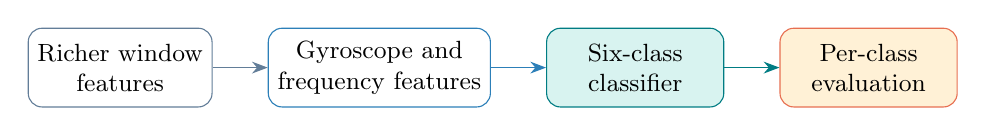
\begin{tikzpicture}[node distance=7mm,every node/.style={font=\small,align=center}]
    \node[draw=muted,fill=white,rounded corners=5pt,minimum width=2.25cm,minimum height=1cm] (a) {Richer window\\features};
    \node<2->[draw=sky,fill=white,rounded corners=5pt,minimum width=2.25cm,minimum height=1cm,right=of a] (b) {Gyroscope and\\frequency features};
    \node<3->[draw=teal,fill=softteal,rounded corners=5pt,minimum width=2.25cm,minimum height=1cm,right=of b] (c) {Six-class\\classifier};
    \node<4->[draw=coral,fill=softgold,rounded corners=5pt,minimum width=2.25cm,minimum height=1cm,right=of c] (d) {Per-class\\evaluation};
    \draw<2->[-{Stealth[length=2mm]},muted] (a) -- (b);
    \draw<3->[-{Stealth[length=2mm]},sky] (b) -- (c);
    \draw<4->[-{Stealth[length=2mm]},teal] (c) -- (d);
  \end{tikzpicture}
  \vspace{.65cm}
  \begin{columns}[T,onlytextwidth]
    \begin{column}{.47\textwidth}
      \uncover<2->{\begin{block}{Feature expansion}
        Per-axis means, variance, magnitude energy, and later gyroscope features.
      \end{block}}
    \end{column}
    \begin{column}{.47\textwidth}
      \uncover<3->{\begin{block}{Evaluation expansion}
        Accuracy, macro F1, confusion matrices, and subject-disjoint held-out testing.
      \end{block}}
    \end{column}
  \end{columns}
\end{frame}

\section{References}
\begin{frame}[allowframebreaks]{References}
  \footnotesize
  \begin{thebibliography}{9}
    \bibitem{anguita2013}
    D. Anguita, A. Ghio, L. Oneto, X. Parra, and J. L. Reyes-Ortiz.
    \newblock Human Activity Recognition on Smartphones Using a Multiclass Hardware-Friendly Support Vector Machine.
    \newblock In \emph{Ambient Assisted Living and Home Care}, 2013. DOI: 10.1007/978-3-642-35395-6\_30.

    \bibitem{kwapisz2011}
    J. R. Kwapisz, G. M. Weiss, and S. A. Moore.
    \newblock Activity Recognition Using Cell Phone Accelerometers.
    \newblock \emph{ACM SIGKDD Explorations}, 12(2):74--82, 2011. DOI: 10.1145/1964897.1964918.

    \bibitem{banos2014}
    O. Ba\~nos, J.-M. G\'alvez, M. Damas, H. Pomares, and I. Rojas.
    \newblock Window Size Impact in Human Activity Recognition.
    \newblock \emph{Sensors}, 14(4):6474--6499, 2014. DOI: 10.3390/s140406474.

    \bibitem{basseville1993}
    M. Basseville and I. V. Nikiforov.
    \newblock \emph{Detection of Abrupt Changes: Theory and Application}.
    \newblock Prentice Hall, 1993.

  \end{thebibliography}
\end{frame}

% 18
\begin{frame}[plain]
  \vspace{1.4cm}
  \begin{center}
    {\Huge\bfseries\color{ink}Thank you}\\[.35cm]
    {\Large\color{muted}Questions and discussion}\\[.8cm]
    
\begin{tikzpicture}
      \draw[teal,line width=1.3pt] (0,0) .. controls (.45,.65) and (.85,-.55) .. (1.3,.18)
      .. controls (1.65,.72) and (2.05,-.3) .. (2.55,.35)
      .. controls (2.95,.86) and (3.35,-.18) .. (3.85,.22);
    \end{tikzpicture}
  \end{center}
\end{frame}

\end{document}
